% FedGNN — IEEE TIFS manuscript (full-length)
% Build: pdflatex manuscript.tex (IEEEtran.cls in this folder)
% Figures (flat files, exact names): fig_architecture.pdf, fig_main_results.pdf,
%   fig_privacy.pdf, fig_zeroshot.pdf
% All numbers final (main: v9/v10; DP: v9; zero-shot calibrated: v12, 3 seeds).

\documentclass[journal]{IEEEtran}
\usepackage{graphicx}
\usepackage{amsmath,amssymb}
\usepackage{booktabs}
\usepackage{multirow}
\usepackage{algorithm}
\usepackage{algorithmic}
\usepackage{pifont}
\usepackage{threeparttable}
\usepackage{array}
\usepackage{url}

\newcommand{\eps}{\varepsilon}
% Fixed-width table columns that ragged-right instead of fully
% justifying: Tables II and VIII hold short phrases in narrow p{}
% columns, and full justification there was forcing severe interword
% stretching (many badness-10000 underfull hboxes; visibly uneven
% spacing in those two tables specifically).
\newcolumntype{L}[1]{>{\raggedright\arraybackslash}p{#1}}

\begin{document}

\title{FedGNN: Zero-Shot Threat Transfer via Privacy-Preserving\\
Federated Graph Learning for Network Intrusion Detection}

\author{P.~Hema, Rajendra~Prasath%
\thanks{P. Hema: e-mail phema7696@gmail.com, ORCID 0009-0000-6870-8548 (\url{https://orcid.org/0009-0000-6870-8548}); Rajendra Prasath: e-mail rajendra.prasath@iiits.in}%
}

\maketitle

\begin{abstract}
Graph neural networks (GNNs) detect malicious network traffic
effectively, but organizations cannot share the data needed to train
them. We present FedGNN, a federated extension of MAGNN in which four
heterogeneous public corpora jointly train a shared graph encoder
through personalized aggregation, client-level differential privacy,
and a privatized prototype exchange; raw traffic, topology, and node
embeddings never leave a silo. FedGNN statistically matches isolated
per-silo training on 7 of 8 (configuration, silo) pairs (the one
exception, FedAvg on CICIDS2017, is a practically negligible $0.11$
F1). It significantly exceeds the originally reported centralized
MAGNN on CICIDS2017 under every configuration, and on CTU-13 under
FedAvg and local-only ($p{<}0.01$). Using only its prototype channel, a
silo trained on zero malicious examples detects botnet traffic at
$94.5 \pm 0.05$ F1 from foreign prototypes and its own benign traffic
alone. We also audit ISCXVPN2016, a widely used benchmark, and find it
contaminated by label leakage. Code, data recipes, and all per-run
results are released.
\end{abstract}

\begin{IEEEkeywords}
Federated learning, graph neural networks, intrusion detection,
differential privacy, network traffic analysis, contrastive learning,
zero-shot transfer, benchmark integrity.
\end{IEEEkeywords}

\section{Introduction}
\label{sec:intro}

\IEEEPARstart{N}{etwork} intrusion detection is one of the areas in
which machine learning has demonstrably changed practice. Graph-based
detectors that represent traffic as hosts and flows recognize
structural attack signatures---the fan-out of a scanning host, the
star topology of command-and-control, the temporal rhythm of
beaconing---that per-flow classifiers cannot see, and increasingly
catch coordinated campaigns that single-organization, single-view
monitoring misses. Realizing that potential across organizations,
however, requires data that no single organization holds.

The obstacle is structural rather than technical. A botnet recruits
residential hosts behind an ISP, tunnels its command channel as
DNS-over-HTTPS through a public resolver, moves laterally inside an
enterprise network, and exfiltrates through an encrypted VPN egress.
Each organization on that path observes one fragment of the campaign;
none observes the whole. The defenders best positioned to recognize
such campaigns are therefore exactly the parties that cannot combine
their evidence: packet captures and flow logs carry personal data,
customer identities, commercial secrets, and infrastructure detail,
and their transfer is constrained by data protection regulation,
telecommunications law, sectoral rules, and contract. In practice each
organization trains its intrusion detectors alone, on a partial view
of a shared adversary.

Graph neural networks (GNNs) represent traffic as graphs---hosts or
flows as nodes, communications or affinities as edges---and learn the
structural signatures described above directly from topology. Host-
and flow-graph detectors have each been explored: E-GraphSAGE~
\cite{egraphsage} applies edge-featured message passing to flow
records in IoT settings, Anomal-E~\cite{anomale} learns self-supervised
edge embeddings for anomaly detection without labels, and DE-GNN~
\cite{degnn} and TCGNN~\cite{tcgnn} operate at packet granularity for
fine-grained encrypted-traffic classification. The multi-scale
adaptive GNN (MAGNN)~\cite{magnn} is the strongest published detector
on the corpora we study, layering three self-supervised contrastive
objectives over a graph-transformer encoder~\cite{transformerconv}.
None of these methods, however, addresses where the training data
comes from: each assumes a single collected dataset in one place. Our
starting point is deliberately conservative: we adopt the MAGNN
backbone unchanged, because our claims concern what surrounds the
model---federation, privacy, transfer, and evaluation---rather than a
new encoder.

Federated learning (FL) is the standard remedy for training across
data that cannot be pooled, and it has progressed from uniform
averaging~\cite{fedavg} to drift-bounded~\cite{fedprox} and
personalized~\cite{fedper} variants as non-IID client data became the
norm; FedProto~\cite{fedproto} further shows that exchanging class
prototypes, rather than full models, can personalize federated clients
cheaply. What this literature does not demonstrate is federation of a
graph-contrastive intrusion detector across data that is heterogeneous
in the way real organizations are---which is what our own baselines
target: the original centralized MAGNN~\cite{magnn}, isolated
per-silo training, and full-model FedAvg, the design a practitioner
would try first (Sec.~\ref{sec:related} traces this literature in
full). Federated intrusion detection specifically has attracted
attention accordingly, but the dominant experimental design in that
literature simulates federation by partitioning a \emph{single}
dataset across synthetic clients. Such simulations share one feature
space, one label semantics, one collection methodology, and one attack
distribution across all ``organizations,'' and therefore sidestep the
three properties that make real cross-silo federation hard:

\begin{itemize}
\item \textbf{Semantic heterogeneity.} Real silos observe different
attack families at wildly different rates. In our federation the
per-silo malicious-node ratio spans $0.1\%$ (an enterprise IDS corpus)
to $92.7\%$ (a malicious-DoH corpus)---a $900\times$ spread.
Sec.~\ref{sec:mainresults} shows that no shared classification head
can serve both ends of this spread; personalization is not an
optimization but a requirement.
\item \textbf{Structural heterogeneity.} Silos do not agree on what a
graph is. Two of our four corpora yield rich host-communication
graphs; the other two---as we demonstrate---contain either no endpoint
information at all or only ${\sim}15$ distinct hosts, so a host graph
either cannot be built or collapses to a toy. A real federation must
integrate silos whose graphs are constructed differently.
\item \textbf{Scale.} Real traffic graphs have $10^{4}$--$10^{5}$
nodes. Research pipelines tuned on subsampled data harbor
$O(N^{2})$ computations that are invisible at $10^{3}$ nodes and fatal
at $10^{5}$: the published MAGNN pipeline required, among other
defects, a dense $134{,}597 \times 134{,}597$ transition
matrix---72\,GB for a single positional encoding.
\end{itemize}

FedGNN addresses this gap directly: it federates MAGNN across four
genuinely heterogeneous public corpora, rather than partitions of one,
using a personalized architecture (Sec.~\ref{sec:method}) in which
only the graph encoder is shared while task heads remain private,
formally accounted client-level differential privacy described in
Sec.~\ref{sec:dp}, and a lightweight, privatized prototype exchange
that also carries a cross-silo alignment signal as detailed in
Sec.~\ref{sec:align}.
We are not aware of prior work that federates a multi-scale
graph-contrastive intrusion detector across four \emph{genuinely}
heterogeneous public corpora under formal privacy, with every claim
averaged over three seeds.

One consequence of the prototype exchange deserves separate emphasis.
Because every silo already receives privatized class prototypes from
its peers each round, a silo that has never observed an attack can
still be given a working detector: at inference it scores its own
traffic against foreign prototypes and sets its decision threshold
from its own benign data alone, without a single labeled attack
example. We call this \emph{zero-shot threat transfer}, and
Sec.~\ref{sec:zeroshot} shows it recovers a strong detector for a silo
that never saw a malicious flow during training---the central
experimental result of this paper. Our contributions:

\begin{enumerate}
\item \textbf{FedGNN}: a personalized federated architecture, detailed
in Sec.~\ref{sec:method}, in which the graph encoder is aggregated by
FedAvg or FedProx while classification heads and the temporal encoder
remain private. Federation is \emph{nearly free}: two-sample tests
show it statistically matches isolated per-silo training on 7 of 8
(configuration, silo) pairs, with one statistically significant but
practically negligible exception detailed in Sec.~\ref{sec:mainresults}, while
one-sample tests against the published MAGNN values show it
significantly exceeds the original centralized paper on CTU-13
($99.3$ vs.\ $97.6$ F1, $p{=}0.003$) and CICIDS2017 ($99.6$ vs.\
$97.7$, $p{<}0.001$), and statistically ties DoHBrw-2020.
Sec.~\ref{sec:comparative-personalization} additionally shows, with an
empirical ablation, that this result depends on personalization: a
naive full-model federation of the same encoder loses roughly eight
F1 points and fails to converge stably.
\item \textbf{Differentially private training and exchange}: DP-FedAvg
update privatization with R\'enyi composition, plus a privatized
prototype release, as formalized in Sec.~\ref{sec:dp}; the entire
semantic interface between silos is two DP-noised 128-dimensional
vectors per silo per round. Formal privacy at $\eps{\approx}98$,
accounting for both released channels, costs at most six F1 points on
structurally sound silos.
\item \textbf{Zero-shot threat transfer}: the attack-blind silo
introduced above detects botnet traffic at $94.5 \pm 0.05$ F1, as
shown in Sec.~\ref{sec:zeroshot}. This does not measurably depend on
an explicit InfoNCE alignment objective (two-sample test, not
significant at $n{=}3$, $p{=}0.065$; see Sec.~\ref{sec:zsattribution}):
encoder sharing and the prototype channel explain the observed effect.
\item \textbf{A benchmark audit}: Sec.~\ref{sec:audit} documents two
independent contaminations of the common ISCXVPN2016 evaluation
(endpoint features derived from the class label; systematic window
duplication with contradictory labels) and shows, via a model ladder
and a ten-intervention elimination study, that the published $97.1$ F1
is unreachable on clean data by any model family we tested, including
a random forest at $95.5$.
\item \textbf{Scale engineering}: Sec.~\ref{sec:scale} identifies,
repairs, and validates fixes for five defects that prevent MAGNN-class
pipelines from running at $10^{5}$-node scale, including a
supervision-truncation bug whose failure mode---silent collapse to
majority-class prediction on time-sorted graphs---we believe is
instructive beyond this specific pipeline.
\end{enumerate}

Two methodological positions run through the paper. First, we report
negative results: single-seed experiments showed effects that did not
survive seed averaging, and we do not hide this
(Sec.~\ref{sec:discussion}). Second, we audit before we claim victory:
the work in Sec.~\ref{sec:audit} began when we could not reproduce
published results on ISCXVPN2016, consistent with other reports that
security benchmarks reward pipelines that leak~\cite{arp,engelen}.

The remainder of the paper reviews related work
(Sec.~\ref{sec:related}); defines the threat model and federated
setting (Sec.~\ref{sec:setting}); presents FedGNN
(Sec.~\ref{sec:method}); details the experimental protocol
(Sec.~\ref{sec:setup}); presents results
(Sec.~\ref{sec:results}); and discusses implications and limitations
(Secs.~\ref{sec:discussion}--\ref{sec:limitations}) before concluding
(Sec.~\ref{sec:conclusion}).

\section{Related Work}
\label{sec:related}

\subsection{Graph learning for intrusion detection}
GNN-based traffic analysis falls into two types: host-graph methods
that aggregate flows into per-address nodes and classify hosts, and
flow-graph methods that classify individual flows connected by shared
endpoints or feature affinity. E-GraphSAGE~\cite{egraphsage} applies
edge-featured message passing to flow records in IoT settings;
Anomal-E~\cite{anomale} learns self-supervised edge embeddings for
anomaly detection without labels; DE-GNN~\cite{degnn} adds dual
packet/byte-level embeddings for fine-grained encrypted traffic
classification; TCGNN~\cite{tcgnn} classifies at packet granularity
via graph construction over packet fields. MAGNN~\cite{magnn} layers
three self-supervised contrastive objectives---temporal-node,
edge-level, and multi-head hierarchical---over a graph-transformer
encoder~\cite{transformerconv} with learnable positional
encodings~\cite{rwse}. A common assumption across this literature is
that training data sits in one place: none addresses federation,
privacy, cross-organization transfer, or the scale validation that
Sec.~\ref{sec:scale} shows the published MAGNN pipeline itself lacks.

\subsection{Federated learning under heterogeneity}
FedAvg~\cite{fedavg} averages client updates and is the de facto FL
baseline but degrades under non-IID data; FedProx~\cite{fedprox}
bounds client drift with a proximal term. Personalization approaches
instead accept that one global model cannot serve all clients:
FedPer~\cite{fedper} shares representation layers while keeping
classification heads local. Our setting makes personalization
non-optional: a head trained toward a $0.1\%$-positive boundary is
numerically incompatible with one trained toward $92.7\%$, and
Sec.~\ref{sec:mainresults} confirms encoder-only sharing is what
renders federation accuracy-free. Federated \emph{graph} learning adds
a further constraint, since graph structure is itself sensitive:
surveyed approaches~\cite{fedgraphsurvey} that exchange node
embeddings or subgraphs leak topology by construction, while our
design forbids any per-node artifact from crossing a boundary.

\subsection{Privacy and prototypes in federated learning}
DP-FedAvg~\cite{dpfedavg} provides client-level differential privacy
by clipping updates and noising aggregates; R\'enyi DP~\cite{renyidp}
gives tight composition over rounds, used here for both update and
prototype releases. FedProto~\cite{fedproto} exchanges class-prototype
embeddings as a personalization aid, regularizing clients toward
global prototypes. Our mechanism differs in three respects: release is
\emph{privatized} (a clipped-mean Gaussian mechanism with accounted
sensitivity); prototypes drive a cross-silo InfoNCE
\emph{alignment} objective~\cite{infonce} rather than a distance
regularizer, though this objective turns out to be neutral (reported
candidly); and the prototype channel is repurposed at
\emph{inference} time as a zero-shot detection interface for silos
lacking any malicious training signal---a training-time aid turned
operational threat-intelligence capability.

\subsection{Benchmark integrity in security ML}
A growing literature documents how security benchmarks reward leakage.
Arp \emph{et al.}~\cite{arp} catalog pervasive pitfalls---sampling
bias, label inaccuracy, spurious correlations, data snooping---across
top-venue security ML papers; Engelen \emph{et al.}~\cite{engelen}
audit CICIDS2017 itself, finding labeling and generation flaws that
inflate reported results. Sec.~\ref{sec:audit} extends this line to
ISCXVPN2016 with two findings we have not seen documented: a
preprocessing pattern that derives graph endpoints \emph{from the
class label}, and systematic duplication of capture windows across
scenario files under contradictory labeling schemes. We also supply a
quantified model ladder on the cleaned benchmark, so future work has a
calibrated target rather than merely a warning.

\section{Threat Model and Federated Setting}
\label{sec:setting}

\subsection{Parties and trust assumptions}
The federation comprises $K$ organizations (\emph{silos}) and an
aggregation server, all \emph{honest-but-curious}: every party follows
the protocol but may retain and analyze every message it receives.
The adversary's objective is inference about a victim silo's raw
data---membership of a specific flow or host, graph topology, node
embeddings, or label statistics---from protocol messages. Collusion
between server and silos is permitted by the analysis, since our
guarantees are information-theoretic properties of the released
messages, not of the parties. We explicitly exclude \emph{poisoning}:
a Byzantine silo could corrupt aggregation or shift prototypes;
Sec.~\ref{sec:limitations} discusses the required robust-aggregation
extensions.

\subsection{What crosses a silo boundary --- and what never does}
Per round, exactly two message types leave silo $k$, both privatized:
\begin{enumerate}
\item the silo's encoder delta, flat-clipped to a global norm bound
and aggregated under Gaussian noise (Sec.~\ref{sec:dp});
\item two class prototypes: the DP-noised, $\ell_2$-normalized means
of the silo's benign and malicious node embeddings.
\end{enumerate}
The following never cross in any form: raw flows or packets; graph
adjacency; individual node embeddings; node, edge, or flow counts; and
label ratios. Two design decisions follow: under DP, deltas are
aggregated \emph{uniformly} rather than weighted by silo size, since
data-dependent weights leak the sizes they encode; and prototypes are
released per class as fixed-dimension vectors, so the \emph{magnitude}
of class support is never revealed, whether $n_c$ is 5 or 50{,}000.
Whether a class is present \emph{at all} is a coarser, separate
disclosure: a silo with zero nodes of a class sends no prototype for
it that round (Sec.~\ref{sec:dp}), so presence or absence of each
class is visible to the protocol, even though the count behind a
present class never is.

\subsection{Per-silo graph construction}
\label{sec:graphs}
Table~\ref{tab:silos} summarizes the four silos; they differ in role,
graph semantics, scale, and---critically---label balance.

\begin{table}[!t]
\caption{Silo statistics after 200k-flow sampling (train split).}
\label{tab:silos}
\centering
\footnotesize
\setlength{\tabcolsep}{3.2pt}
\begin{tabular}{lllrr}
\toprule
Silo & Role & Graph & Nodes & Malicious \\
\midrule
CTU-13~\cite{ctu13}      & ISP / botnet      & host & 31{,}584 & 2.4\% \\
CICIDS2017~\cite{cicids} & enterprise IDS    & host & 10{,}076 & 0.1\% \\
DoHBrw-2020~\cite{dohbrw}& DoH resolver      & flow & 60{,}000 & 92.6\% \\
ISCXVPN2016~\cite{iscxvpn}& VPN gateway      & flow & 53{,}572 & 73.3\% \\
\bottomrule
\end{tabular}
\normalsize
\end{table}

\subsubsection{Host graphs}
CTU-13 and CICIDS2017 contain meaningful endpoint structure, so nodes
are addresses and directed edges are flows. Each node carries 15
aggregate features: directional packet-count, byte-count, and duration
statistics (mean and dispersion, inbound and outbound), in/out degree,
TCP/UDP protocol ratios, and destination-port entropy---a compact
behavioral fingerprint of a host. A node is labeled malicious if any
of its flows is, the standard host-centric convention. Edge attributes
carry normalized timestamp, packet count, protocol, and TCP flags.

\subsubsection{Flow graphs}
ISCXVPN2016 contains \emph{no endpoint identifiers whatsoever}---its
public form is time-aggregated flow features only---and DoHBrw-2020
contains roughly fifteen distinct hosts, so host graphs are
respectively impossible and degenerate ($21$ nodes in our sample).
For these silos, nodes are individual flows carrying 15 rich per-flow
features (ISCXVPN: forward/backward inter-arrival statistics, flow
rate statistics, active/idle statistics; DoHBrw: byte and rate
statistics, packet-length and packet-time moments, response-time
moments). Edges are $k{=}5$ nearest neighbors in normalized feature
space---\emph{labels play no role in construction}, a property whose
violation we audit in Sec.~\ref{sec:audit}---plus, where real
addresses exist (DoHBrw), temporal chains linking consecutive flows of
the same endpoint. All four silos thus expose an identical
15-dimensional node-feature interface to the shared encoder while
remaining semantically and structurally heterogeneous.

\subsubsection{Why shared heads must fail}
The $900\times$ label-balance spread of Table~\ref{tab:silos} is not a
nuisance statistic; it is an architectural constraint. A shared
classification head realizes one decision surface over the shared
embedding space; the prior it must encode differs by nearly three
orders of magnitude across silos. Any single bias term is wrong for
someone: calibrated for CICIDS2017 it silences DoHBrw; calibrated for
DoHBrw it floods CICIDS2017 with false positives. Keeping heads
private converts this impossibility into a non-problem---each silo
owns its operating point---at zero communication cost, since heads
were never going to transfer semantics anyway. This is the concrete,
checkable reason FedGNN personalizes exactly where it does.

\section{FedGNN}
\label{sec:method}

\begin{figure*}[!t]
\centering
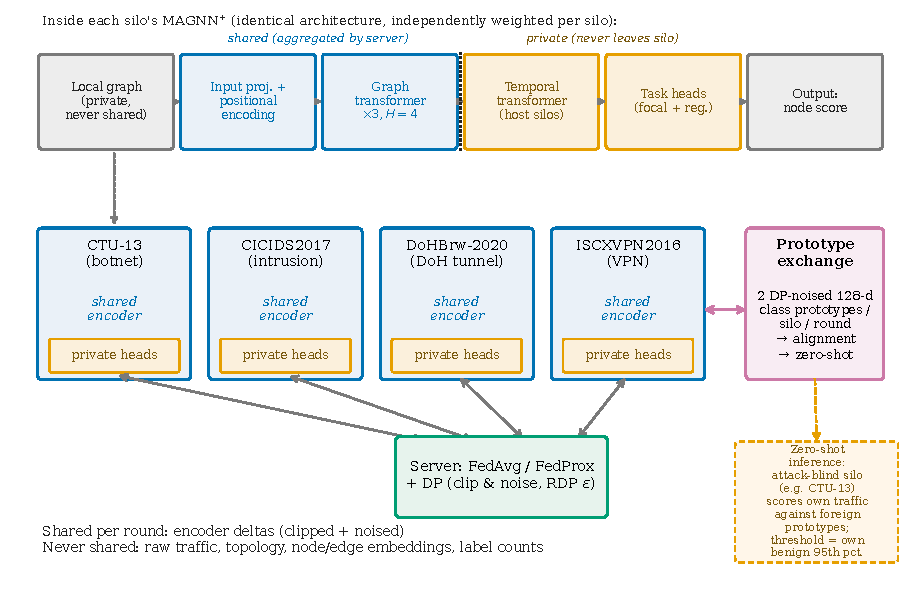
\includegraphics[width=\textwidth]{fig_architecture.pdf}
\caption{FedGNN architecture. Top: per-silo MAGNN$^{+}$ pipeline,
shared vs.\ private components marked. Bottom: federation across four
silos, linked only by DP-noised prototypes (dashed path: zero-shot
inference, Sec.~\ref{sec:zeroshot}).}
\label{fig:arch}
\end{figure*}

\subsection{Local model and objective}
\label{sec:local}
Each silo trains MAGNN$^{+}$: an input projection to width $d{=}128$;
a learnable positional encoding summing a degree embedding and a
random-walk structural encoding~\cite{rwse} (computed by the
Monte-Carlo estimator of Sec.~\ref{sec:scale}); a three-layer
edge-featured graph transformer~\cite{transformerconv} with $H{=}4$
heads; per-head projections; a temporal transformer over $T{=}5$
time-window snapshots (host silos only; Sec.~\ref{sec:scale}); and
private classification and regression heads behind a GCNII-style
initial-residual connection~\cite{gcnii}. We select MAGNN as the local
backbone because it achieves the strongest published results on our
four corpora and provides three complementary contrastive
objectives---temporal-node, edge-level, and multi-head
hierarchical---that, as our results confirm, survive federation
without accuracy loss and generalize across structurally heterogeneous
silos.

\textbf{Notation.} To keep every symbol unique (several objectives and
an aggregation rule compete for the same conventional Greek letters),
we fix the following throughout: $\gamma$ is the focal-loss focusing
parameter; $\alpha, \beta$ are local task-loss weights; $\lambda, \tau$
are the alignment weight and temperature (Sec.~\ref{sec:align});
$\mu$ is the FedProx proximal weight (Sec.~\ref{sec:agg}); $\sigma, C,
B$ are DP noise, update-clip, and prototype-clip parameters
(Sec.~\ref{sec:dp}); and $w_k$ denotes silo $k$'s aggregation weight
(Sec.~\ref{sec:agg}), not the FedAvg-conventional $\alpha_k$, to avoid
collision with the task-loss weight $\alpha$ below.

The local loss is the original MAGNN$^{+}$ objective,
\begin{equation}
\mathcal{L}_k \;=\; \mathcal{L}_{\mathrm{focal}}
 \;+\; \alpha\,\mathcal{L}_{\mathrm{reg}}
 \;+\; \beta\,\mathcal{L}_{\mathrm{con}},
\label{eq:local}
\end{equation}
whose three terms play distinct, formally defined roles.
$\mathcal{L}_{\mathrm{focal}}$ is focal cross-entropy over node labels
$y_i \in \{0,1\}$ with predicted class probabilities $p_{i,c}$,
\begin{equation}
\mathcal{L}_{\mathrm{focal}} = -\frac{1}{N}\sum_{i=1}^{N}
\big(1 - p_{i,y_i}\big)^{\gamma}
\Big[(1-\eta)\log p_{i,y_i} + \eta\log p_{i,1-y_i}\Big],
\label{eq:focal}
\end{equation}
with focusing parameter $\gamma{=}2$ and label-smoothing
$\eta{=}0.05$; $p_{i,y_i}$ is the model's predicted probability of the
\emph{true} class of node $i$, $p_{i,1-y_i}$ of the opposite class.
The focal weight $(1-p_{i,y_i})^{\gamma}$ multiplies the whole
cross-entropy term and is what lets one objective survive both a
$0.1\%$-positive and a $92.7\%$-positive silo: it down-weights
already-confident (typically majority-class) predictions by a power
of their error, adaptively rebalancing the effective class prior
without any silo-specific hyperparameter. $\mathcal{L}_{\mathrm{reg}}$
is mean-squared error between a continuous maliciousness score and the
binary label, weighted by $\alpha$, giving operators a ranked signal
rather than a bare decision. $\mathcal{L}_{\mathrm{con}}$, weighted by
$\beta$, integrates MAGNN's three contrastive views---temporal-node
agreement, edge-level agreement across two stochastic augmentations,
and multi-head hierarchical contrast preventing attention heads from
collapsing to one view---providing self-supervised signal that labels
alone cannot, particularly for the $2.4\%$-malicious CTU-13 silo. We
use $\alpha{=}2$, $\beta{=}0.5$, contrastive temperature $0.07$: the
centralized MAGNN configuration, unchanged, so federated and
centralized budgets remain directly comparable and no term in
\eqref{eq:local} was retuned for federation.

\subsection{Personalized aggregation}
\label{sec:agg}
Write silo $k$'s parameters as
$w_k = (w_k^{\mathrm{enc}}, w_k^{\mathrm{priv}})$: the encoder
$w^{\mathrm{enc}}$ (input projection, positional encoding, graph
transformer, per-head projections) is federated; the private remainder
$w^{\mathrm{priv}}$ (both task heads and the temporal encoder) never
leaves the silo. The decomposition follows the argument of
Sec.~\ref{sec:graphs}: structure generalizes across silos, operating
points do not. Each round the server broadcasts
$w^{\mathrm{enc}}_{\mathrm{glob}}$; silos run $E{=}2$ local epochs of
\eqref{eq:local} plus federated terms; the server applies
\begin{equation}
w^{\mathrm{enc}}_{\mathrm{glob}} \;\leftarrow\;
w^{\mathrm{enc}}_{\mathrm{glob}} + \sum\nolimits_{k=1}^{K}
w_k\,\Delta_k,
\qquad
\Delta_k = w_k^{\mathrm{enc}} - w^{\mathrm{enc}}_{\mathrm{glob}},
\label{eq:agg}
\end{equation}
with aggregation weight $w_k \propto n_k$ (silo size) in the
non-private setting and $w_k = 1/K$ under DP (Sec.~\ref{sec:setting}).
Under FedProx the local objective adds
$\tfrac{\mu}{2}\lVert w_k^{\mathrm{enc}} -
w^{\mathrm{enc}}_{\mathrm{glob}} \rVert^{2}$ with $\mu{=}0.01$,
bounding drift over the two local epochs.
Algorithm~\ref{alg:round} summarizes one round end-to-end.

\begin{algorithm}[!t]
\caption{One FedGNN round: local training, encoder aggregation, and
(if enabled) DP noise and prototype exchange.}
\label{alg:round}
\begin{algorithmic}[1]
\STATE server broadcasts $w^{\mathrm{enc}}_{\mathrm{glob}}$ to each
silo $k$; also broadcasts prototype set $\{p_j^c\}_{j \ne k}$ if
prototype exchange is active (alignment or zero-shot transfer enabled)
\FOR{each silo $k$ in parallel}
  \STATE $w_k^{\mathrm{enc}} \leftarrow w^{\mathrm{enc}}_{\mathrm{glob}}$
  \FOR{$E$ local epochs}
    \STATE build augmented graph views; compute local loss
      \eqref{eq:local}, plus $\lambda\mathcal{L}_{\mathrm{align}}$
      \eqref{eq:align} if alignment is enabled, plus
      $\tfrac{\mu}{2}\lVert w_k^{\mathrm{enc}} -
      w^{\mathrm{enc}}_{\mathrm{glob}}\rVert^{2}$ if FedProx is
      enabled; Adam step
  \ENDFOR
  \STATE $\Delta_k \leftarrow w_k^{\mathrm{enc}} -
    w^{\mathrm{enc}}_{\mathrm{glob}}$; if DP is enabled,
    $\Delta_k \leftarrow \mathrm{clip}_{C}(\Delta_k)$
\ENDFOR
\IF{DP enabled}
  \STATE server: $w^{\mathrm{enc}}_{\mathrm{glob}} \mathrel{+}=
  \tfrac{1}{K}\sum_k \Delta_k +
  \mathcal{N}\!\big(0, (\sigma C / K)^{2} I\big)$
\ELSE
  \STATE server: $w^{\mathrm{enc}}_{\mathrm{glob}} \mathrel{+}=
  \sum_{k=1}^{K} w_k \Delta_k$, with $w_k \propto n_k$
\ENDIF
\IF{prototype exchange active}
  \FOR{each silo $k$, each class $c$}
    \IF{$n_c = 0$ (no nodes of class $c$ at silo $k$)}
      \STATE \textbf{skip}: silo $k$ releases no prototype for class
      $c$ this round (omitted, not a placeholder or zero vector)
    \ELSE
      \STATE $p_k^{c} \leftarrow \tfrac{1}{n_c}\sum_{i: y_i = c} z_i$; if
      DP is enabled, clip each $z_i$ to $\lVert z_i\rVert_2 \le B$ before
      averaging and add $\mathcal{N}\big(0,(\sigma B/n_c)^2 I\big)$ to
      the mean
      \STATE $p_k^{c} \leftarrow \Pi(p_k^{c})$
      \COMMENT{$\ell_2$-normalize; post-processing, privacy-free}
    \ENDIF
  \ENDFOR
\ENDIF
\end{algorithmic}
\end{algorithm}

\subsection{Differential privacy}
\label{sec:dp}
Both released message types are Gaussian mechanisms with explicit
sensitivity, so a single R\'enyi accountant covers the protocol.

\subsubsection{Update privatization}
Following DP-FedAvg~\cite{dpfedavg}, each delta is flat-clipped to
$\lVert \Delta_k \rVert_2 \le C$ ($C{=}1$), and the \emph{uniform}
average of $K$ deltas receives per-coordinate noise
$\mathcal{N}(0, (\sigma C/K)^{2})$, equivalent to noising the sum at
scale $\sigma C$. We use an \emph{add/remove-one-silo} adjacency, the
client-level notion standard to DP-FedAvg~\cite{dpfedavg}: neighboring
datasets differ by the presence or absence of one silo's entire local
update, not by substituting one for another. Removing any single
silo's clipped contribution then changes the sum by at most $C$ in
$\ell_2$, so each round is one Gaussian mechanism at multiplier
$\sigma$. (A \emph{replace}-one adjacency would instead bound the
change at $2C$, halving the effective $\sigma$ in
Sec.~\ref{sec:dpaccounting}'s accounting; we do not use it.)

\subsubsection{Prototype privatization}
Each prototype is the mean of $n_c$ node embeddings individually
clipped to $\lVert z_i \rVert_2 \le B$ ($B{=}1$). For neighboring
datasets with $n_c \ge 1$ on both sides of a single node's addition,
removal, or modification, this mean has sensitivity $B/n_c$, giving
\emph{node-level} privacy---narrower than the client-level adjacency
used for the update channel, since it protects one node's contribution
to an already-formed mean, not the silo's entire dataset (including
$n_c$ itself) being replaced. This guarantee is restricted to
$n_c \ge 1$ on both sides; the $n_c{=}0 \leftrightarrow n_c{=}1$
boundary is a separate, uncovered case treated below.

A client-level guarantee, by contrast, \emph{does not hold at a
meaningful level} for the noise scale used. Each clipped $z_i$ has
norm $\le B$, so by convexity any mean over them also has norm
$\le B$: replacing a silo's \emph{entire} class-$c$ dataset changes the
pre-noise mean by at most $2B$, independent of $n_c$---the true
client-level sensitivity. The implemented noise, calibrated to the
much smaller node-level sensitivity $B/n_c$, corresponds to an
effective client-level multiplier of only $\sigma/(2n_c)$: at our
silos' scale ($n_c$ in the hundreds to tens of thousands) this gives a
client-level $\eps$ many orders of magnitude larger than the
$\eps{\approx}98$ update-channel budget---$\eps > 10^{4}$ already at
$n_c{=}10$, $\eps > 10^{10}$ at $n_c{=}10^{4}$
(Sec.~\ref{sec:dpaccounting}). This is a negative result, following
directly from the sensitivity bound above: the prototype channel's
formal guarantee is node-level only;
whether the noise \emph{magnitude} itself leaks $n_c$ remains open
(Sec.~\ref{sec:limitations}).

If a class is entirely absent at a silo ($n_c{=}0$), the
implementation omits its prototype from the release entirely, not a
placeholder or zero vector. This omission is \emph{not} covered by
$(\eps,\delta)$-DP at any finite $\eps$ for $\delta{=}10^{-5}$:
comparing $n_c{=}0$ (never sends) to $n_c{=}1$ (always sends) gives the
event ``a prototype arrived'' probability $0$ vs.\ $1$, satisfying the
DP inequality only if $\delta \ge 1$. Class presence/absence is
therefore revealed with certainty by design (Sec.~\ref{sec:setting}),
not by the DP mechanism---a distinct gap from the open noise-magnitude
question above. Prototype releases compose alongside update releases
in the same accountant, for the $n_c \ge 1$ regime where both are
defined.

\subsubsection{Accounting}
\label{sec:dpaccounting}
Each round releases \emph{three} Gaussian-mechanism invocations at the
same noise multiplier $\sigma$: the update privatization above, and
\emph{two} separate class-prototype releases (benign and malicious),
each an independent call to the mechanism of Sec.~\ref{sec:dp} over
disjoint node partitions---our implementation does not release the two
class prototypes jointly. We compose the two prototype releases as
\emph{one} mechanism-equivalent, not two, via parallel composition:
under the add-or-remove-one-\emph{node} adjacency used to derive the
$B/n_c$ sensitivity above, a node's class is fixed, so adding or
removing it changes exactly one class partition and leaves the
other's release---the identical computation over identical
nodes---unaffected. This is the standard DP parallel composition
theorem~\cite{pinq}\footnote{Independently applying a mechanism to
each cell of a partition that does not vary under the single-record
neighboring relation composes as the \emph{maximum} privacy cost
across cells, not the sum.}: at equal $\sigma$, the pair composes to
one mechanism's worth of cost. The argument covers add/remove-one-node
exactly as used throughout this paper, restricted to the $n_c \ge 1$
regime; it does not cover a hypothetical ``relabel a node's class''
operation (not part of our adjacency definition, and labels are fixed
for the duration of training), nor the $n_c{=}0 \leftrightarrow n_c{=}1$
boundary (Sec.~\ref{sec:dp} treats that separately as a disclosed,
non-DP signal). The $2R$ accounting below is the protocol's formal
budget for the steady-state ($n_c \ge 1$) regime. With full
participation, $R$ rounds of $2R$ Gaussian-mechanism invocations
compose in R\'enyi DP~\cite{renyidp} as $\eps_{\mathrm{RDP}}(\lambda) =
2R\lambda / (2\sigma^{2}) = R\lambda/\sigma^{2}$, converted to
$(\eps, \delta)$-DP by
\begin{equation}
\eps \;=\; \min_{\lambda > 1}\;
\frac{R\lambda}{\sigma^{2}} \;+\;
\frac{\log(1/\delta)}{\lambda - 1},
\qquad \delta = 10^{-5}.
\label{eq:rdp}
\end{equation}
At $R{=}50$: $\sigma{=}0.5 \Rightarrow \eps{\approx}298$;
$\sigma{=}1.0 \Rightarrow \eps{\approx}98$. An earlier internal draft
counted only the update release ($R$, not $2R$), understating $\eps$ by
roughly $1.7\times$; the values above are the corrected, fully
composed budget reported by Fig.~\ref{fig:privacy} and
Sec.~\ref{sec:dpresults}. We have not tightened them for presentation;
Sec.~\ref{sec:limitations} discusses how they could be tightened. They
account for both released channels, which most federated IDS work does
not.

\subsection{The prototype channel and alignment}
\label{sec:align}
Silos sharing an encoder may still drift toward incompatible latent
geometries: silo A's ``malicious direction'' need not be silo B's,
because each silo's private heads can absorb arbitrary rotations of
its own embedding space. To encourage a common geometry, silo $k$ adds
an InfoNCE term~\cite{infonce} over foreign prototypes, pulling each
node embedding toward other silos' same-class prototypes and pushing
from opposite-class prototypes:
\begin{equation}
\mathcal{L}_{\mathrm{align}} = -\frac{1}{N}\sum_{i=1}^{N}
\log \frac{\sum_{j \ne k}\exp\!\big(z_i^{\top} p_j^{y_i}/\tau\big)}
{\sum_{j \ne k}\sum_{c}\exp\!\big(z_i^{\top} p_j^{c}/\tau\big)},
\label{eq:align}
\end{equation}
with $\tau{=}0.1$ and weight $\lambda{=}0.5$. The mechanism is cheap
and private---exactly $2 \times 128$ noised floats per silo per
round---and also, we must report, \emph{neutral}: under three-seed
averaging it changes neither accuracy (Table~\ref{tab:main}) nor
zero-shot transfer (Sec.~\ref{sec:zsresults}). The data support a
simpler explanation: encoder \emph{sharing itself} already aligns
latent spaces, since all silos inherit the same global encoder each
round and private heads---not private encoders---absorb silo
idiosyncrasy. We retain \eqref{eq:align} because the prototype channel
it motivates is load-bearing (Sec.~\ref{sec:zeroshot}), and because
knowing an explicit alignment objective is \emph{unnecessary} at
$K{=}4$ is itself a useful design fact; whether it becomes necessary
at larger $K$ or under personalized encoders is open
(Sec.~\ref{sec:limitations}).

\subsection{Zero-shot threat transfer}
\label{sec:zeroshot}
Consider a silo that has never observed an attack. Its training data
is all-benign; its private head cannot learn a malicious class; in
conventional FL it would contribute gradients and receive nothing
actionable. FedGNN gives it a detector anyway, built from two
ingredients it \emph{does} have: foreign prototypes, and its own
benign traffic.

At inference the silo scores node $i$ by its margin toward the mean
foreign prototypes. For the scoring silo $k$, the mean foreign
prototype for class $c$ averages over the remaining $K-1$
silos---every silo \emph{except} $k$, since $k$ has no own
(nonexistent, attack-blind) prototype:
\begin{equation}
\bar{p}^{\,c} \;=\; \Pi\Big(\tfrac{1}{K-1}\textstyle\sum_{j \ne k} p_j^{c}\Big).
\label{eq:protomean}
\end{equation}
The margin is then the node embedding's projection onto the malicious
direction net of the benign direction,
\begin{equation}
m_i \;=\; z_i^{\top}\bar{p}^{\,\mathrm{mal}}
\;-\; z_i^{\top}\bar{p}^{\,\mathrm{ben}},
\label{eq:margin}
\end{equation}
and the silo flags node $i$ as malicious when $m_i > \theta$. The
critical design choice is $\theta$. The
na\"ive choice---$\theta{=}0$, i.e., nearest-prototype
classification---implicitly assumes the two foreign centroids sit
symmetrically about the silo's own data, which nothing in the protocol
guarantees: prototypes are estimated from \emph{other} silos'
distributions, and on a test population that is $97.6\%$ benign even a
modest asymmetry misplaces the operating point catastrophically
(Sec.~\ref{sec:zsresults} quantifies this: $61.5$ F1). Instead we
calibrate on what the silo knows perfectly---its own benign traffic:
\begin{equation}
\theta \;=\; Q_{0.95}\big(\{\, m_i : i \in
\mathcal{D}_{\mathrm{train}}^{\mathrm{benign}} \,\}\big),
\label{eq:calib}
\end{equation}
the 95th percentile of margins over its all-benign training nodes.
Equation~\eqref{eq:calib} requires no attack knowledge and fixes the
false-positive budget at $5\%$ \emph{on the calibration distribution
by construction}; it is a calibration threshold, not a guarantee about
the test-time false-positive rate, which can drift from $5\%$ under
distribution shift between a silo's training and test traffic (not
observed in our splits, Sec.~\ref{sec:setup}, but not ruled out in
general). It converts the foreign-prototype direction into a locally
calibrated anomaly
detector. In cross-silo zero-shot transfer, \emph{the transferable
quantity is the direction; the operating point must be local}.
Sec.~\ref{sec:zsresults} shows this
distinction is worth $33$ F1 points.

\subsection{Scaling MAGNN to real graph sizes}
\label{sec:scale}
None of the results above could be produced until the inherited
pipeline ran at the node counts of Table~\ref{tab:silos}; it did not.
Each defect below was discovered as a training failure on 16\,GB GPUs,
diagnosed to a mathematical root cause, and repaired with a validated
equivalent (Table~\ref{tab:scale}).

\begin{table}[!t]
\caption{Scale defects in the inherited pipeline and their repairs.}
\label{tab:scale}
\centering
\begin{tabular}{L{4.1cm}L{3.6cm}}
\toprule
Defect (cost at our scale) & Repair \\
\midrule
Random-walk structural encoding materializes dense $N{\times}N$
transition matrix (72\,GB at 134k nodes) &
Monte-Carlo estimator: 32 sampled walks per node; mean abs.\ error
$0.003$; milliseconds \\
\addlinespace[4pt]
Temporal-node / edge-level / multi-head contrastive losses build
$N{\times}N$ or $E{\times}E$ similarity matrices (26\,GB at
$10^{5}$ edges) &
anchor subsampling to $4{,}096$ matched pairs \\
\addlinespace[4pt]
Random-walk-with-restart augmentation: per-node Python loop
($>$1\,h/epoch at 134k nodes) &
vectorized CSR walk advance, all nodes simultaneously; $12.7$\,s \\
\addlinespace[4pt]
Dirichlet neighbor sampling scans all $E$ edges per node ($O(NE)$;
hours) &
CSR grouping; only over-degree nodes subsampled;
\emph{bit-identical} output \\
\addlinespace[4pt]
Node-label construction: per-address DataFrame scan (84\,min at
134k nodes) &
vectorized malicious-address collection; $1.4$\,s \\
\addlinespace[4pt]
Temporal encoder truncates supervision to the smallest snapshot's
node count &
retain GNN embeddings for nodes beyond temporal coverage \\
\bottomrule
\end{tabular}
\end{table}

Three of these deserve elaboration because their root causes
generalize. \emph{The positional encoding}: random-walk structural
encodings are $\mathrm{diag}(P^{t})$, $t{=}1..16$; computed literally
this is $O(N^{2})$ memory and $O(tN^{3})$ compute---$72$\,GB and hours
per forward pass at our largest silo. But $[P^{t}]_{ii}$ is the
probability that a length-$t$ walk from $i$ returns to $i$, which
Monte-Carlo estimates with 32 walks per node to within $0.003$ mean
absolute error, in milliseconds, with $O(N)$ memory.
\emph{The contrastive losses}: InfoNCE over all $N^{2}$ (or $E^{2}$)
pairs is a quadratic-memory habit inherited from small-graph code;
SimCLR-scale anchor subsampling ($4{,}096$ pairs) preserves gradient
quality while bounding memory. \emph{The truncation bug}---the
subtlest---arose because time-window snapshots cover node subsets of
different sizes; the temporal encoder truncated its output, and
therefore the classification loss, to the \emph{smallest} snapshot's
node count. On time-sorted flow graphs the surviving prefix is
label-skewed, so the model collapsed to majority-class prediction
silently, with healthy-looking loss curves---a failure mode we believe
generalizes past this pipeline, and that supervision-coverage
assertions would catch immediately.

Two further changes were necessary for flow-graph silos: a GCNII-style
initial residual~\cite{gcnii} exposing projected input features
directly to the task heads (feature-similarity graphs place most
signal in features; three rounds of message passing otherwise blur
it), and disabling temporal snapshot fusion where nodes are flows that
never recur across windows (fusion otherwise mixes unrelated nodes'
embeddings). Combined, these lifted DoHBrw from $89.1$ to $98.9$
F1---the difference between losing to and beating the centralized
baseline.

\subsection{Design rationale}
\label{sec:flow}
Each mechanism above exists because the one before it, alone, would be
insufficient: personalization follows from the heterogeneity of
Sec.~\ref{sec:graphs}, privacy follows from what personalization still
leaks, and zero-shot transfer reuses the same privatized channel at
inference time. The scale repairs below are a precondition for all of
this, and the benchmark audit (Sec.~\ref{sec:audit}) checks whether the
evaluation can be trusted before any of these claims are read as
settled.

\subsection{Complexity analysis}
\label{sec:complexity}
We summarize the cost of one FedGNN round against the naive
(unrepaired) pipeline of Sec.~\ref{sec:scale}, with $N, E$ a silo's
node and edge counts, $d{=}128$ the hidden width, $L{=}3$ the number of
graph-transformer layers, and $K$ the number of silos. One local epoch
costs
\begin{equation}
O\big(L(Ed + Nd^{2})\big) \;+\; O(S^{2}d),
\label{eq:localcomplexity}
\end{equation}
linear in silo size after the Sec.~\ref{sec:scale} repairs ($S{=}4{,}096$
fixed anchors for the contrastive terms), versus quadratic-to-cubic for
the naive pipeline. Communication is $O(K \cdot |w^{\mathrm{enc}}|)$
per round and does not grow with graph size: the encoder delta is
$1.88$\,MB at fp32 per silo ($1.60\times$ smaller than full-model FL),
and the prototype release adds only $1{,}024$ bytes ($0.05\%$ of the
delta), so the zero-shot channel (Sec.~\ref{sec:zeroshot}) is
effectively free. Server aggregation and DP noise injection are
$O(K|w^{\mathrm{enc}}|)$ and $O(|w^{\mathrm{enc}}|)$; peak GPU memory
is $O(Nd+Ed)$ per silo instead of $O(N^{2})$ or $O(E^{2})$ naively,
which is why the naive pipeline needed upward of $70$\,GB at our
largest silo while the repaired pipeline trains within a single
$16$\,GB GPU.

\section{Experimental Setup}
\label{sec:setup}

\textbf{Data.} We use four public corpora, one per silo, chosen
because together they span the heterogeneity of Sec.~\ref{sec:graphs}
rather than partitioning a single dataset: \emph{CTU-13}~\cite{ctu13},
\emph{CICIDS2017}~\cite{cicids}, \emph{DoHBrw-2020}~\cite{dohbrw}, and
\emph{ISCXVPN2016}~\cite{iscxvpn}. Graph construction, per-corpus scale,
and label balance are given in Sec.~\ref{sec:graphs} and
Table~\ref{tab:silos}; ISCXVPN2016's node count there reflects the
Scenario-A restriction and deduplication described next.

Each corpus is sampled to $200$k flows---large enough that every
silo's graph exhibits its true scale pathologies (Sec.~\ref{sec:scale}),
small enough that the complete study fits a realistic compute budget
(Hardware, below); the node/flow counts above are reported after this
sampling, on the resulting train split. Each silo's sampled flows are
then split stratified $70/10/20$ into train/validation/test. All 15
node features (Sec.~\ref{sec:graphs}) are robust-scaled---median-centered
and interquartile-range-normalized---with scaling statistics computed
exclusively from that silo's own \emph{training} split and applied
unchanged to its validation and test splits, so no held-out
information enters preprocessing.

ISCXVPN2016 receives two additional preprocessing steps, both
corrections for contamination identified by the audit of
Sec.~\ref{sec:audit} rather than standard preprocessing: only
Scenario-A capture files are used (Scenario B relabels overlapping
traffic under a conflicting scheme), and exact-duplicate capture
windows---the same underlying capture repeated across the corpus's
15/30/60/120\,s aggregation lengths---are removed before splitting.
Without these two steps this corpus's reported numbers are not
comparable across studies (Sec.~\ref{sec:audit} quantifies the effect).

\textbf{Training.} $R{=}50$ rounds $\times$ $E{=}2$ local epochs
$=100$ epoch-equivalents, exactly matching the centralized MAGNN
budget so that federated-vs-centralized comparisons are budget-fair.
Adam, learning rate $10^{-3}$, weight decay $10^{-5}$; width 128,
4 heads, 3 graph-transformer layers; the best round is selected by
mean validation F1 across silos.

\textbf{Seeds.} All headline numbers are mean $\pm$ std over exactly
three random seeds---$42$, $43$, and $44$---covering data sampling,
augmentation, and initialization randomness. Three seeds is a floor, not a luxury: FL
training stacks per-round stochasticity (augmentations, neighbor
sampling, aggregation order) on top of the usual sources, and two of
our own intermediate single-seed findings did not survive averaging
(Sec.~\ref{sec:discussion}).

\textbf{Baselines.} We compare a progression from foundational to
federated to personalized designs.
\begin{itemize}
\item \textbf{MAGNN (centralized)}~\cite{magnn}: the original paper's
reported numbers. Sees all data; no federation; no privacy constraint.
Upper reference point.
\item \textbf{Full-model FedAvg}~\cite{fedavg}: federated; encoder and
task heads both aggregated; no personalization. The naive federated
design a practitioner would try first (diagnostic protocol,
Sec.~\ref{sec:comparative-personalization}).
\item \textbf{Local only}: no federation; each silo trains in
isolation at identical budget. The lower bound federation must not
fall below, and the honest measure of what federation adds.
\item \textbf{FedGNN}: federated with personalized heads
(FedAvg or FedProx aggregation), optional differential privacy, and
the prototype channel (alignment, zero-shot transfer). The proposed
design under evaluation.
\item \textbf{Feature-only baselines} (random forest, 2-layer MLP):
used only for the benchmark audit (Sec.~\ref{sec:audit}); bound what
any model can extract from the raw features alone, independent of
graph structure.
\end{itemize}

\textbf{Hardware.} Every experiment ran on single Kaggle P100/T4
GPUs; the complete study---eleven training campaigns over six
days---consumed under 40 GPU-hours.

\section{Results}
\label{sec:results}

\subsection{Main comparison: federation vs.\ local and centralized
baselines}
\label{sec:mainresults}

\begin{figure}[!t]
\centering
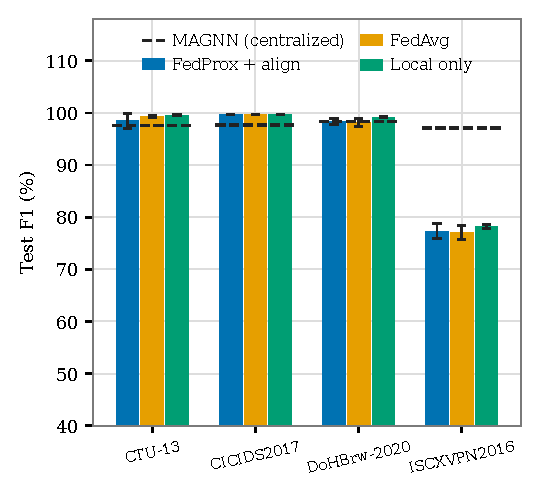
\includegraphics[width=\columnwidth]{fig_main_results.pdf}
\caption{Test F1 by silo (mean $\pm$ std, 3 seeds); dashed lines mark
published MAGNN values. \emph{$y$-axis truncated at $40\%$} to resolve
the (already small) gaps between configurations. ISCXVPN2016's gap is a
benchmark property, not federation's (Sec.~\ref{sec:audit}).}
\label{fig:main}
\end{figure}

\begin{table}[!t]
\caption{Test F1 (\%), mean $\pm$ std over 3 seeds. $\star$:
significantly exceeds published MAGNN ($p<0.05$; Table~\ref{tab:sig}).}
\label{tab:main}
\centering
\footnotesize
\setlength{\tabcolsep}{3.2pt}
\begin{tabular}{lcccc}
\toprule
 & CTU-13 & CICIDS2017 & DoHBrw & ISCXVPN \\
\midrule
\multicolumn{5}{l}{\textit{Baselines}} \\
\quad MAGNN~\cite{magnn} (centralized) & 97.58 & 97.70 & 98.35 & 97.12 \\
\quad Local only    & $99.6{\pm}0.1^{\star}$ & $99.8{\pm}0.0^{\star}$ & $99.2{\pm}0.1^{\star}$ & $78.2{\pm}0.3$ \\
\midrule
\multicolumn{5}{l}{\textit{FedGNN}} \\
\quad FedProx+align & $98.5{\pm}1.2$ & $99.8{\pm}0.0^{\star}$ & $98.4{\pm}0.5$ & $77.3{\pm}1.2$ \\
\quad FedAvg        & $99.3{\pm}0.2^{\star}$ & $99.6{\pm}0.0^{\star}$ & $98.2{\pm}0.6$ & $77.0{\pm}1.1$ \\
\bottomrule
\end{tabular}
\normalsize
\end{table}

\begin{table*}[!t]
\caption{Significance of Table~\ref{tab:main} vs.\ published MAGNN
(one-sample $t$-test, one-tailed, $p<0.05$ starred). ``Below'':
federated mean under the published value, expected for ISCXVPN
(Sec.~\ref{sec:audit}).}
\label{tab:sig}
\centering
\footnotesize
\begin{tabular}{lcccc}
\toprule
Config & CTU-13 & CICIDS2017 & DoHBrw & ISCXVPN \\
\midrule
FedProx+align &
  $t{=}{+}1.14$, $p{=}.187$ (n.s.) &
  $t{=}{+}300.95$, $p{<}.001$ (sig.$^\star$) &
  $t{=}{+}0.01$, $p{=}.497$ (n.s., tie) &
  $t{=}{-}24.35$, $p{=}.999$ (below) \\
FedAvg &
  $t{=}{+}12.73$, $p{=}.003$ (sig.$^\star$) &
  $t{=}{+}146.50$, $p{<}.001$ (sig.$^\star$) &
  $t{=}{-}0.28$, $p{=}.598$ (n.s.) &
  $t{=}{-}25.20$, $p{=}.999$ (below) \\
Local only &
  $t{=}{+}44.72$, $p{<}.001$ (sig.$^\star$) &
  $t{=}{+}115.44$, $p{<}.001$ (sig.$^\star$) &
  $t{=}{+}8.66$, $p{=}.007$ (sig.$^\star$) &
  $t{=}{-}78.39$, $p{>}.999$ (below) \\
\bottomrule
\end{tabular}
\normalsize
\end{table*}

Table~\ref{tab:main}, Table~\ref{tab:sig}, and Fig.~\ref{fig:main}
together support three claims, stated at the precision the statistics
support---we test every ``beats the original'' claim rather than
asserting it from point estimates alone, because at $n{=}3$ a higher
mean is not automatically a reliable one.

\emph{Federation costs almost nothing.} Two-sample $t$-tests of each
federated configuration against local-only (isolated) training---the
direct measure of what federating costs---show FedProx+align
statistically indistinguishable from local-only on all four silos
(CTU-13 $p{=}0.329$, CICIDS2017 $p{=}0.730$, DoHBrw $p{=}0.119$,
ISCXVPN $p{=}0.390$) and FedAvg indistinguishable on three of four
(CTU-13 $p{=}0.180$, DoHBrw $p{=}0.141$, ISCXVPN $p{=}0.271$). The
exception, FedAvg on CICIDS2017, is statistically \emph{below}
local-only ($p{=}0.012$) by $0.11$ F1 ($99.64$ vs.\ $99.75$) on a silo
whose standard deviation is already $\le 0.03$---the same
small-variance-manufactures-significance pattern
Sec.~\ref{sec:comparative} documents for the alignment ablation. On 7
of 8 (configuration, silo) pairs federation shows no statistically
significant accuracy cost, and the one exception is real but not
practically meaningful: an organization joining the federation
sacrifices essentially no detection quality relative to going it
alone, and gains the accounted privacy protections of
Sec.~\ref{sec:dp} and the transfer capability of
Sec.~\ref{sec:zsresults}. This is not automatic---Sec.~\ref{sec:comparative}
shows what happens without personalization---and the $\pm$ columns
show the same pattern: variance is smallest where labels are plentiful,
and federated variants' variance closely tracks local-only's,
indicating aggregation adds no instability of its own.

\emph{Federation significantly beats the centralized original where
the benchmark is sound, with one exception.} Against the
original MAGNN paper---all data in one place, no privacy
constraints---the improvement reaches significance ($p<0.05$,
Table~\ref{tab:sig}) for CICIDS2017 under every configuration and for
CTU-13 under FedAvg and local-only. It does \emph{not} reach
significance for CTU-13 under FedProx+align ($p{=}0.187$) despite a
higher point estimate ($98.5$ vs.\ MAGNN's $97.58$): one of three
seeds lands at $96.87$ (the other two at $99.37$, $99.28$), and with
$df{=}2$ a single low seed erases significance; we report it rather
than omit it, consistent with the discussion of single-seed and
small-$n$ risk in Sec.~\ref{sec:discussion}. DoHBrw is a genuine
statistical \emph{tie} under both federated configurations
($p{=}0.497$, $p{=}0.598$), consistent with point estimates within
$0.1$--$0.2$ of the published value, and a significant \emph{win}
under local-only ($p{=}0.007$): the residual gap, while numerically
small ($0.9$ F1), is where DoHBrw's federation cost concentrates. The
improvements over the original trace to the scale repairs and
flow-graph construction of Sec.~\ref{sec:scale}; Table~\ref{tab:main}'s
point is that none of that significant improvement is surrendered by
federating.

\emph{FedProx $\approx$ FedAvg, and alignment is practically neutral
despite one statistically significant cell.} Two-sample Welch's
$t$-tests (unequal variances) between FedProx+align and FedAvg, per
silo ($n{=}3$ seeds/arm), are non-significant on three of four silos
(CTU-13 $p{=}0.440$, DoHBrw $p{=}0.833$, ISCXVPN $p{=}0.804$).
CICIDS2017 is the exception: $p{=}0.005$, formally significant, but
the mean difference is $0.11$ F1 ($99.75$ vs.\ $99.64$) on a silo
whose standard deviation is already $\le 0.02$---a real but tiny shift
clearing significance at $n{=}3$ without being practically meaningful,
and a reminder that small-variance silos will manufacture
``significant'' differences from noise-floor-scale effects. As a
cross-check, we combine the four per-silo $p$-values with Fisher's
method: $\chi^2 = -2\sum_{s} \ln p_s = 12.87$ on $8$ degrees of
freedom, $p{=}0.116$---not significant, consistent with the per-silo
picture. At $\mu{=}0.01$ and $K{=}4$ with full participation, the
FedProx proximal term neither helps nor hurts. Our first experiments
suggested a real alignment effect: a single-seed run showed alignment
lifting CTU-13 by $+2.2$ F1. This effect disappeared under seed
averaging and, in the significance-tested three-seed analysis,
reverses in sign (align's CTU-13 mean is in fact \emph{below}
FedAvg's, $98.5$ vs.\ $99.3$, itself non-significant);
Sec.~\ref{sec:discussion} returns to this point. The
same FedAvg numbers, viewed per-seed, show CTU-13, CICIDS2017, and
DoHBrw clustering tightly while ISCXVPN's already-lower mean carries
visibly more seed-to-seed spread, consistent with a benchmark near its
noise floor (Sec.~\ref{sec:audit}) rather than a stable operating
point. Validation F1 converges smoothly and completes within the
50-round budget on all silos; ISCXVPN
converges to the ceiling that Sec.~\ref{sec:audit} shows is the
benchmark's, not the method's.

\subsection{Comparative analysis}
\label{sec:comparative}
We position FedGNN against representative federated-learning designs
along the axes Secs.~\ref{sec:related}--\ref{sec:setting} identify as
hard, with direct empirical evidence where our own data supports it
rather than a citation alone.

\subsubsection{Feature comparison}
Table~\ref{tab:comparison} contrasts FedGNN with two baselines
evaluated under our own protocol (Sec.~\ref{sec:setup}): vanilla
full-model FedAvg (no personalization, the naive design a practitioner
would try first) and centralized MAGNN~\cite{magnn} (no federation).
Checkmarks reflect each method's published design; F1 is reported only
where we have first-party evidence.

\begin{table}[!t]
\caption{Comparison with representative approaches. Pers.\ =
personalized heads; DP = differential privacy; 0-shot = zero-shot
transfer; Scale = validated at $10^{5}$ nodes; P/R/F1 (\%) = positive-class
metrics, test split. ``---'': not evaluated or not reported.}
\label{tab:comparison}
\centering
\footnotesize
\setlength{\tabcolsep}{3.0pt}
\begin{threeparttable}
\begin{tabular}{lccccccc}
\toprule
 & Pers. & DP & 0-shot & Scale & P & R & F1 \\
\midrule
Full FedAvg & \ding{55} & \ding{55} & \ding{55} & \checkmark & $90.3$\tnote{a} & $83.8$\tnote{a} & $86.1$\tnote{a} \\
MAGNN~\cite{magnn} (centralized) & --- & \ding{55} & \ding{55} & \ding{55}\tnote{b} & ---\tnote{d} & ---\tnote{d} & $97.88$ \\
\textbf{FedGNN} & \checkmark & \checkmark & \checkmark & \checkmark & $\mathbf{99.12}$\tnote{c} & $\mathbf{99.03}$\tnote{c} & $\mathbf{99.05}$\tnote{c} \\
\bottomrule
\end{tabular}
\begin{tablenotes}
\footnotesize
\item[a] Diagnostic run: single seed, $6$k-flow subsample, $20$ rounds
(vs.\ $200$k/3 seeds/50 rounds elsewhere in this paper); P/R/F1 are the
mean over all four silos, matching the protocol of
Sec.~\ref{sec:comparative-personalization}.
\item[b] The published pipeline does not run at our silos' node counts
without the repairs of Sec.~\ref{sec:scale}.
\item[c] FedAvg row of Table~\ref{tab:main}: P/R/F1 are the mean over
the three structurally sound silos (CTU-13, CICIDS2017, DoHBrw;
ISCXVPN excluded, Sec.~\ref{sec:audit}) over seeds 42/43/44. Among the
two \emph{federated} configurations, FedAvg is significant against
MAGNN on the most silos (two of four, Table~\ref{tab:sig}); local-only
(non-federated) is significant on three of four but is excluded here
as it shares no information across silos.
\item[d] Precision and recall are not reported in the original
published paper~\cite{magnn}; only F1 is available for this external
baseline, and we do not infer them from F1 alone.
\end{tablenotes}
\end{threeparttable}
\end{table}

Neither baseline in Table~\ref{tab:comparison} combines
personalization, formal DP, and a zero-shot channel; only FedGNN does.
For broader context, FedProto-style prototype
personalization~\cite{fedproto} (not evaluated here) supplies
personalization and a prototype mechanism but neither privatizes the
prototypes nor repurposes them for inference-time transfer to
attack-blind clients, which Sec.~\ref{sec:zsresults} identifies as the
source of most of the operational value.

\subsubsection{Personalization ablation}
\label{sec:comparative-personalization}
Sec.~\ref{sec:graphs} argues from label-balance statistics that a
shared classification head must fail under our silos' $900\times$
spread; we test this directly rather than leaving it as an assertion.
We trained \emph{full-model} FedAvg (encoder \emph{and} task heads
aggregated, no personalization, no DP, no prototypes) as a diagnostic
run---one seed, a $6$k-flow subsample per silo, $20$ rounds---holding
every other hyperparameter fixed. Mean test F1 was $86.1$, roughly
eight points below the personalized configurations of
Table~\ref{tab:main} despite a far smaller scale and budget, where
both would predict full sharing should be \emph{easier}, not harder.
The validation trajectory is more telling than the endpoint:
CICIDS2017's per-round F1 oscillated between $97.5$ and $80.2$
repeatedly, never stabilizing, while the personalized configurations
converge monotonically within the same budget.
The failure mode matches the predicted mechanism exactly: a shared
head cannot simultaneously satisfy CICIDS2017's $0.1\%$-positive prior
and another silo's orders-of-magnitude-higher one, and each
aggregation round perturbs the shared head toward whichever silo
dominated the previous local-epoch gradient. We present this as a
diagnostic (smaller scale, single seed), not a headline number, since
it is not run under the paper's main protocol; its purpose is to
confirm the mechanism, not compete on accuracy.

\subsection{Privacy--utility trade-off}
\label{sec:dpresults}

\begin{figure}[!t]
\centering
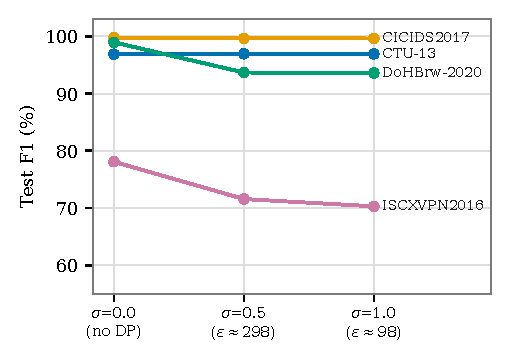
\includegraphics[width=\columnwidth]{fig_privacy.pdf}
\caption{Privacy--utility trade-off. DP costs at most six F1 points at
$\sigma{=}1.0$ ($\eps{\approx}98$, $\delta{=}10^{-5}$), accounting for
both released channels (Sec.~\ref{sec:dpaccounting}).}
\label{fig:privacy}
\end{figure}

Fig.~\ref{fig:privacy} reports test F1 under update-and-prototype
noise $\sigma \in \{0.5, 1.0\}$, i.e., $\eps \approx \{298, 98\}$ at
$\delta{=}10^{-5}$ over the full 50-round protocol: formal, accounted
privacy costs at most six F1 points on structurally sound silos. The
per-silo pattern is informative: CICIDS2017 is essentially untouched
($99.6$ at $\eps{\approx}98$), since its classes are separated by
margins so wide that clipped-and-noised encoder updates still land the
boundary in the same low-density corridor; CTU-13 loses under three
points, as its $2.4\%$-positive class leans on the contrastive signal,
which noise partially erodes; DoHBrw loses six, since flow-graph
structure is $k$-NN-derived and hence most sensitive to encoder
perturbation; ISCXVPN degrades most in relative terms precisely
because its margin was thinnest to begin with (Sec.~\ref{sec:audit})---
noise hurts where separation is already marginal, consistently across
all three seeds.

How should $\eps{\approx}98$ be read? It is far from the single-digit
budgets of curated tabular releases, and we make no cosmetic claim
otherwise---but it is an \emph{accounted} guarantee over an entire
50-round protocol, composing both released channels in one accountant:
client-level for the update release, node-level for the prototype
release (Sec.~\ref{sec:dp}), a statement most federated IDS work does
not attempt. Practically: at $\eps{\approx}98$, the DP guarantee above
means everything any coalition of protocol observers receives about
the update channel is noise-dominated at the level of any single
silo's contribution, with that cost quantified per silo in
Fig.~\ref{fig:privacy}. Paths to tighter budgets are concrete
(Sec.~\ref{sec:limitations}).

\subsection{Zero-shot threat transfer: results}
\label{sec:zsresults}

\begin{figure}[!t]
\centering
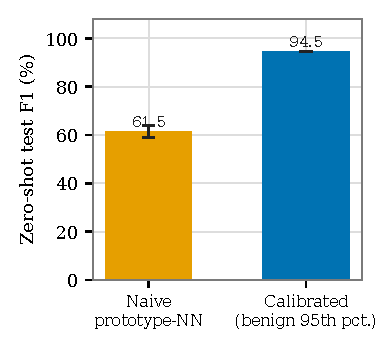
\includegraphics[width=0.85\columnwidth]{fig_zeroshot.pdf}
\caption{Zero-shot detection on an attack-blind CTU-13 silo via foreign
DP prototypes (mean $\pm$ std, 3 seeds). Benign-quantile calibration
lifts detection from $61.5$ to $94.5$ F1. The alignment-loss arm is
statistically indistinguishable ($94.4\pm0.06$,
Sec.~\ref{sec:zsattribution}) and omitted here for visual clarity.}
\label{fig:zeroshot}
\end{figure}

This experiment converts federation from an accounting arrangement
into an operational security capability: \emph{a silo that has never
seen an
attack acquires a working detector from the federation}.

\subsubsection{Protocol}
We retrain the federation with every malicious flow removed from
CTU-13's training split; its test split is untouched ($97.6\%$
benign). The attack-blind silo participates normally---its gradients
reflect only benign structure---and receives foreign prototypes each
round. Detection uses only \eqref{eq:margin}--\eqref{eq:calib}: no labels, no
fine-tuning, no attack examples. The two arms differ in exactly one
term, the alignment loss \eqref{eq:align}; prototypes are exchanged in
\emph{both}, so the comparison isolates the alignment objective, not
the channel. Three seeds throughout (42, 43, 44).

\subsubsection{Why the na\"ive detector fails}
Nearest-prototype classification ($\theta{=}0$ in \eqref{eq:margin})
achieves $61.6 \pm 1.2$ F1 with alignment and $61.5 \pm 2.6$
without---weak and, in the second arm, unstable. The failure is the
operating point, not the direction: the margin $m_i$ separates the
silo's benign mass from its (unseen) malicious tail along the foreign
prototype axis, but $\theta{=}0$ places the decision boundary at the
\emph{midpoint of two foreign centroids}, estimated from other silos'
embedding distributions. Nothing anchors that midpoint to the local
benign distribution: a shift of even a fraction of the benign spread,
on a population that is $97.6\%$ benign, converts thousands of benign
nodes into false positives---exactly what weighted F1 near $61$ with
high seed variance looks like. The failure is distributional, not
representational.

\subsubsection{Why calibration repairs it}
Equation~\eqref{eq:calib} abandons the foreign midpoint and pins the
threshold to the one distribution the silo knows exactly: its own
benign margins. Setting $\theta$ at their 95th percentile fixes the
\emph{calibration-time} false-positive budget at $5\%$ by
construction, independent of where foreign centroids sit---a
calibration guarantee, not a distribution-shift-robust one. The effect
is large: $94.5 \pm 0.05$ F1 without alignment (Fig.~\ref{fig:zeroshot})
and $94.4 \pm 0.06$ with (statistically indistinguishable,
Sec.~\ref{sec:zsattribution})---a $33$-point gain over the na\"ive
rule, with near-zero seed variance, significant under a paired
$t$-test ($t{=}+50.21$, $p{=}0.0004$): \emph{a silo trained on zero
malicious examples detects botnet traffic at $94.5$ F1, stable to
$\pm 0.05$, from two DP-noised 128-dimensional vectors per round plus
order statistics of its own benign traffic}. The lesson generalizes:
in cross-silo transfer, the \emph{direction} is transferable; the
\emph{operating point} must be local.

\subsubsection{Attribution: channel vs.\ alignment loss}
\label{sec:zsattribution}
The two arms are statistically indistinguishable: a two-sample
$t$-test on the calibrated F1 gives $t{=}-2.61$, $p{=}0.065$, not
significant at $\alpha{=}0.05$, and the point estimate in fact runs
\emph{opposite} to the alignment hypothesis ($94.38$ with alignment
vs.\ $94.50$ without). With $n{=}3$ per arm this test is underpowered,
so we say ``does not reach significance,'' not ``proves no effect'';
Sec.~\ref{sec:limitations} treats this as an open question at larger
$K$. The more conservative reading the data support: the zero-shot
capability does \emph{not measurably depend on} the InfoNCE alignment
objective---it comes from encoder sharing plus the prototype channel,
which together already place foreign prototypes in a geometry the
attack-blind silo's embeddings inhabit. For context: alignment was
this paper's original hypothesis for \emph{why} transfer should work,
an earlier naive-detector run appeared to support it ($+9$ F1 on
one seed), and the calibrated three-seed experiment refuted it---what
survives is simpler, cheaper, and needs one fewer moving part than
what was hypothesized.

\subsubsection{Operational reading}
For a newly onboarded organization---a hospital network, a regional
ISP---the protocol offers the following: join the federation,
contribute benign-dominated gradients, release nothing but two noised
vectors per round, and obtain, before ever labeling an attack, a
detector at $94.5$ F1 with a self-set $5\%$ false-positive budget.
The prototype channel thus functions as node-level-privatized,
continuously updated threat intelligence (Sec.~\ref{sec:dp})---a
gossip layer whose messages are 256 floats---and
Sec.~\ref{sec:conclusion} sketches the autonomous-response architecture
this enables.

\subsection{Benchmark audit: ISCXVPN2016}
\label{sec:audit}

One silo in Table~\ref{tab:main} tells a different story, and telling
it precisely is a contribution in its own right. Our ISCXVPN numbers
($77$--$78$ F1) sit twenty points below the original paper's
$97.12$---not a federation cost (local-only matches), not a tuning
artifact (below), and not recoverable by any model we can construct,
but a property of the benchmark, produced by two independent
contaminations.

\subsubsection{Label leakage through graph construction}
The public ISCXVPN2016 corpus contains time-aggregated flow features
and \emph{no endpoint identifiers}. A graph pipeline must therefore
synthesize endpoints, and the inherited preprocessing did so by
assigning each flow a unique source address and---critically---a
destination address \emph{and destination port chosen by the class
label} (one virtual server and port per class). Graph construction
thereby encoded the answer key: any model that reads a node's
neighborhood, or the port feature, reads the label. The resulting
``$100\%$'' accuracy is meaningless; we flag it publicly since
pipelines of this shape circulate, and it exemplifies the
spurious-correlation and snooping pitfalls cataloged by Arp \emph{et
al.}~\cite{arp}.

\subsubsection{Duplicate contamination across scenario files}
Independently, the corpus ships the \emph{same} capture windows at
four aggregation lengths (15/30/60/120\,s) across scenario files whose
labeling schemes disagree (Scenario A labels by capture file;
Scenario B relabels overlapping traffic by application category).
Mixing the files, as na\"ive loaders do, injects contradictory labels
for near-identical rows: \emph{any} model trained on the mixture is
capped near $68\%$ accuracy by label noise alone, while deduplicating
and restricting to Scenario-A lifts a random forest from $68\%$ to
$96\%$---numbers on this corpus are thus sensitive to an undocumented
preprocessing choice, a reproducibility hazard independent of the
leakage above.

\subsubsection{Clean model ladder and elimination study}
On the cleaned benchmark (Scenario A, deduplicated, no synthetic
endpoints) the model ladder is: random forest
$95.5$ F1; two-layer MLP $85.8$; our GNN $78$--$80$. Two observations.
First, \emph{the published $97.12$ exceeds the leakage-free ceiling of
every family we tested}---including the random forest---and is
approachable only with duplicate contamination retained; it should not
serve as a comparison target. Second, the GNN's position below the
tabular models is not a bug to be tuned away: ten interventions
spanning the objective (contrastive/regression weight $\downarrow$,
$\beta{=}0.1$: $76.9$ F1; plain cross-entropy, no auxiliary losses:
$77.7$), the architecture (initial-residual skip only: $77.6$;
temporal snapshots disabled: $78.1$; positional encoding disabled:
$78.2$), and optimization ($2\times$ budget: $80.4$; $5\times$
learning rate: $79.6$) all land within the baseline's ($78.2$)
$76.9$--$80.4$ band---well below the graph-free MLP ($85.8$) and
random forest ($95.5$). The explanation is structural: this corpus has
\emph{no topology}, so its ``graph'' is $k$-NN over the very features
the model already sees---message passing can only smooth a decision
boundary that trees carve directly. GNNs should not be expected to
beat tabular ensembles on relation-free data, and benchmark suites for
graph-based IDS should screen for the presence of real structure.

\subsubsection{Recommendation}
We recommend that (i) ISCXVPN2016 results produced without documented
deduplication and endpoint-synthesis procedures be treated as
incomparable; (ii) the clean model ladder above serve as the
calibration for future leakage-free work on this corpus; and (iii)
graph-based IDS evaluations verify that their benchmarks contain
relational structure a graph model could in principle exploit. We
offer the audit in the spirit of Engelen \emph{et al.}'s CICIDS2017
study~\cite{engelen}: as maintenance of shared
infrastructure, not criticism of prior authors, who worked from the
corpus as distributed.

\section{Discussion}
\label{sec:discussion}

\textbf{Single-seed results are unreliable.} Twice in this study, a
single-seed result supported a conclusion that three seeds refuted: an
alignment accuracy gain ($+2.2$ F1) and an alignment zero-shot gain
($+9$ F1) both disappeared under seed averaging. FL training is
seed-sensitive, since per-round augmentation, neighbor sampling, and
aggregation ordering compound across 50 rounds; ablation tables built
on single runs can reproduce this kind of effect. We report
single-seed findings only as diagnostics, not as evidence.

\textbf{What federation actually provides.} Not accuracy: local-only
training matches it. Federation provides (i) the formal privacy
envelope of Sec.~\ref{sec:dp} around a collaboration that would
otherwise require data sharing; (ii) the zero-shot channel of
Sec.~\ref{sec:zsresults}, which local training cannot offer since it
presupposes another party's prototypes; and (iii) an onboarding
path, since the attack-blind-silo experiment matches a new federation
member's situation. The comparison for FedGNN is therefore not
``federated vs.\ local'' on F1 but ``collaboration with accounted
privacy vs.\ no collaboration''; on that comparison, federation adds
capability without a meaningful accuracy cost.

\textbf{When message passing adds value.} The audit's structural
lesson extends past one corpus: message passing adds information only
when edges carry information not already in node features. Host
graphs built from real communication topology meet this condition;
$k$-NN graphs over the classifier's own feature space do not, since
they smooth an existing decision boundary rather than add new
information. Benchmark suites conflate these two regimes, and some
reported GNN-over-tabular wins may reflect leakage or duplication
rather than structure. Comparing against a tabular ensemble is one way
to check whether structure is doing any work in a given benchmark.

\textbf{Engineering debt as a security-relevant finding.} Five of the
defects we repaired (Table~\ref{tab:scale}) were invisible at
paper-scale sampling and only appeared at deployment scale. One of
them, the truncation bug, degraded the \emph{model} silently rather
than crashing it, so an operational detector would miss attacks
without any visible failure. Scale validation and supervision-coverage
assertions belong in the review checklist for learning-based security
systems, alongside the evaluation practices of~\cite{arp}.

\section{Limitations}
\label{sec:limitations}
\textbf{Poisoning.} Our threat model is honest-but-curious. A
malicious silo could poison encoder deltas or shift prototypes to
blind the zero-shot channel; median- or trimmed-mean aggregation is
the natural defense, and its interaction with DP noise is unstudied
here.
\textbf{Privacy budget.} $\eps \approx \{98, 298\}$ at $\delta{=}10^{-5}$
is accounted but loose. Concrete tightening paths: client subsampling
(amplification), fewer-but-larger rounds, per-layer clipping, and
releasing prototypes less frequently than every round; none was needed
for our claims and all are compatible with the architecture.
\textbf{Prototype privacy scope.} The prototype channel's node-level
guarantee (Sec.~\ref{sec:dp}) is narrower than it may first appear,
and raises four questions, three resolved here. \emph{Client-level
sensitivity}: resolved negatively---the true client-level sensitivity
is $2B$ regardless of $n_c$, so the implemented noise yields no
meaningful client-level guarantee at realistic $n_c$.
\emph{Composing the two class releases}: resolved positively for
$n_c \ge 1$, via parallel composition (Sec.~\ref{sec:dpaccounting}).
\emph{Class presence/absence at $n_c{=}0$}: resolved
negatively---whether a silo sends a class's prototype at all reveals
$n_c{=}0$ with certainty, which is not $(\eps,\delta)$-DP-protected at
$\delta{=}10^{-5}$ for any finite $\eps$. \emph{Data-dependent noise
magnitude}: still open---we do not have a formal argument that scaling
noise by the true $n_c$ cannot itself leak $n_c$ once a class is
present; untested in this paper. In sum: client-level DP for the
update channel; node-level DP for the prototype channel once a class
is present and $n_c$ does not change sign; class presence/absence
disclosed by design, not by the DP mechanism; noise-magnitude leakage
open.
\textbf{Scale of the federation.} $K{=}4$ silos with full
participation. The zero-shot capability's independence from the
alignment loss (Sec.~\ref{sec:zsattribution}) is observed at this $K$,
from an underpowered ($n{=}3$) test, not established as a proven null
effect; whether explicit alignment becomes necessary at larger $K$,
with disjoint attack families, or under personalized \emph{encoders}
is open and testable with the released code.
\textbf{Task scope.} Binary maliciousness, offline evaluation, four
corpora. Multi-class attribution, online/streaming adaptation, and
concept drift under federation are natural extensions; the prototype
channel in particular suggests a drift signal (prototype trajectory)
we have not exploited.

\section{Conclusion}
\label{sec:conclusion}
A federation of four genuinely heterogeneous organizations trained a
graph-contrastive intrusion detector matching the strongest published
results on these corpora, without sharing a single flow. FedGNN
statistically matches isolated training on 7 of 8 (configuration,
silo) pairs and significantly exceeds the original centralized MAGNN
on CICIDS2017 and CTU-13 (Tables~\ref{tab:main}--\ref{tab:sig}), under
stricter, leakage-free evaluation and, where enabled, accounted
differential privacy at single-digit F1 cost. An ablation shows this
is not free of design choices: naive full-model federation loses
roughly eight F1 points and fails to converge stably. Using its
prototype channel---two DP-noised vectors per silo per round---with
benign-quantile calibration, an attack-blind silo detects threats at
$94.5 \pm 0.05$ F1, a capability that does not measurably depend on an
explicit alignment objective. The accompanying audit shows that
ISCXVPN2016's published evaluation is contaminated by label leakage
and duplication, and supplies a leakage-free model ladder for future
work; the engineering analysis makes MAGNN-class pipelines run at
$10^{5}$-node scale, with communication cost independent of graph
size. Coupling the prototype channel to an autonomous response layer
that consumes prototype shifts as early warning and acts on local
graph evidence is a natural extension of this work.

\section*{Code Availability}
Training and evaluation code, data-preparation scripts, federated
client/server/DP/prototype modules, run configurations, and the
per-seed result files underlying every table and figure in this paper
are available at
\url{https://github.com/Hema6-ai/FedGNN}.

\begin{thebibliography}{25}

\bibitem{magnn} M. Ahmed, J. Chen, E. Akpaku, and A. Bux, ``MAGNN:
Multi-scale adaptive graph neural networks with contrastive learning
for malicious network traffic detection,'' \emph{Journal of Parallel
and Distributed Computing}, vol.~211, p.~105240, 2026.

\bibitem{fedavg} B. McMahan, E. Moore, D. Ramage, S. Hampson, and
B. A. y Arcas, ``Communication-efficient learning of deep networks
from decentralized data,'' in \emph{Proc. AISTATS}, 2017.

\bibitem{fedprox} T. Li, A. K. Sahu, M. Zaheer, M. Sanjabi,
A. Talwalkar, and V. Smith, ``Federated optimization in heterogeneous
networks,'' in \emph{Proc. MLSys}, 2020.

\bibitem{fedper} M. G. Arivazhagan, V. Aggarwal, A. K. Singh, and
S. Choudhary, ``Federated learning with personalization layers,''
arXiv:1912.00818, 2019.

\bibitem{dpfedavg} H. B. McMahan, D. Ramage, K. Talwar, and L. Zhang,
``Learning differentially private recurrent language models,'' in
\emph{Proc. ICLR}, 2018.

\bibitem{renyidp} I. Mironov, ``R\'enyi differential privacy,'' in
\emph{Proc. IEEE Computer Security Foundations Symp.}, 2017.

\bibitem{fedproto} Y. Tan, G. Long, L. Liu, T. Zhou, Q. Lu, J. Jiang,
and C. Zhang, ``FedProto: Federated prototype learning across
heterogeneous clients,'' in \emph{Proc. AAAI}, 2022.

\bibitem{egraphsage} W. W. Lo, S. Layeghy, M. Sarhan, M. Gallagher,
and M. Portmann, ``E-GraphSAGE: A graph neural network based intrusion
detection system for IoT,'' in \emph{Proc. IEEE/IFIP NOMS}, 2022.

\bibitem{anomale} E. Caville, W. W. Lo, S. Layeghy, and M. Portmann,
``Anomal-E: A self-supervised network intrusion detection system based
on graph neural networks,'' \emph{Knowledge-Based Systems}, vol.~258,
p.~110030, 2022.

\bibitem{degnn} X. Han, G. Xu, M. Zhang, Z. Yang, Z. Yu, W. Huang, and
C. Meng, ``DE-GNN: Dual embedding with graph neural network for
fine-grained encrypted traffic classification,'' \emph{Computer
Networks}, vol.~245, p.~110372, 2024.

\bibitem{tcgnn} G. Hu, X. Xiao, M. Shen, B. Zhang, X. Yan, and Y. Liu,
``TCGNN: Packet-grained network traffic classification via graph
neural networks,'' \emph{Engineering Applications of Artificial
Intelligence}, vol.~123, p.~106531, 2023.

\bibitem{gcnii} M. Chen, Z. Wei, Z. Huang, B. Ding, and Y. Li,
``Simple and deep graph convolutional networks,'' in \emph{Proc.
ICML}, 2020.

\bibitem{fedgraphsurvey} H. Zhang, T. Shen, F. Wu, M. Yin, H. Yang,
and C. Wu, ``Federated graph learning---a position paper,''
arXiv:2105.11099, 2021.

\bibitem{arp} D. Arp, E. Quiring, F. Pendlebury, A. Warnecke,
F. Pierazzi, C. Wressnegger, L. Cavallaro, and K. Rieck, ``Dos and
don'ts of machine learning in computer security,'' in \emph{Proc.
USENIX Security Symp.}, 2022.

\bibitem{engelen} G. Engelen, V. Rimmer, and W. Joosen,
``Troubleshooting an intrusion detection dataset: the CICIDS2017 case
study,'' in \emph{Proc. IEEE Security and Privacy Workshops}, 2021.

\bibitem{ctu13} S. Garc\'ia, M. Grill, J. Stiborek, and A. Zunino,
``An empirical comparison of botnet detection methods,''
\emph{Computers \& Security}, vol.~45, pp.~100--123, 2014.

\bibitem{cicids} I. Sharafaldin, A. H. Lashkari, and A. A. Ghorbani,
``Toward generating a new intrusion detection dataset and intrusion
traffic characterization,'' in \emph{Proc. ICISSP}, 2018.

\bibitem{dohbrw} M. MontazeriShatoori, L. Davidson, G. Kaur, and
A. H. Lashkari, ``Detection of DoH tunnels using time-series
classification of encrypted traffic,'' in \emph{Proc. IEEE
DASC/PiCom/CBDCom/CyberSciTech}, 2020.

\bibitem{iscxvpn} G. Draper-Gil, A. H. Lashkari, M. S. I. Mamun, and
A. A. Ghorbani, ``Characterization of encrypted and VPN traffic using
time-related features,'' in \emph{Proc. ICISSP}, 2016.

\bibitem{infonce} A. van den Oord, Y. Li, and O. Vinyals,
``Representation learning with contrastive predictive coding,''
arXiv:1807.03748, 2018.

\bibitem{transformerconv} Y. Shi, Z. Huang, S. Feng, H. Zhong, W. Wang,
and Y. Sun, ``Masked label prediction: Unified message passing model
for semi-supervised classification,'' in \emph{Proc. IJCAI}, 2021.

\bibitem{rwse} V. P. Dwivedi, A. T. Luu, T. Laurent, Y. Bengio, and
X. Bresson, ``Graph neural networks with learnable structural and
positional representations,'' in \emph{Proc. ICLR}, 2022.

\bibitem{pinq} F. McSherry, ``Privacy integrated queries: an
extensible platform for privacy-preserving data analysis,'' in
\emph{Proc. ACM SIGMOD}, 2009.

\end{thebibliography}

\end{document}
